\chapter{CƠ SỞ LÝ THUYẾT}

\section{Module ESP8266 Wemos D1}
\subsection{Giới thiệu}
    Module ESP8266 Wemos D1 là phiên bản được thiết kế với hình dạng gần giống board Arduino Uno với trung tâm là module Wifi SoC ESP8266 được xây dựng lại firmware để có thể chạy được với chương trình Arduino.

    ESP8266 Wemos D1 dễ dàng sử dụng và thích hợp với các ứng dụng thu thập dữ liệu và điều khiển qua Wifi.
        \begin{figure}[htp]
            \begin{center}
                \fbox{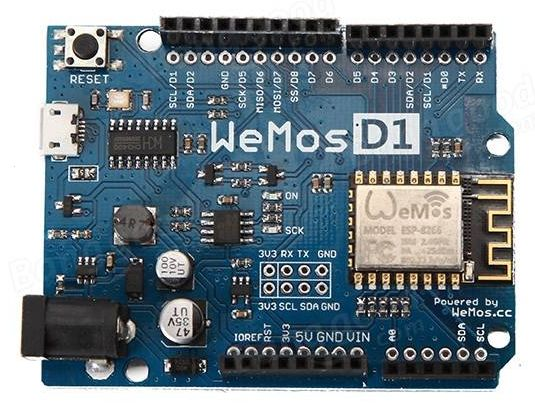
\includegraphics[scale=.5]{esp8266-wemos-d1}}
            \end{center}
            \caption{Module ESP8266 Wemos D1}
            \label{Fig:esp8266-wemos-d1}
        \end{figure}

    Sử dụng cổng Micro USB kết nối module với máy tính để nạp chương trình cho module. Nguồn cấp cho module ESP8266 Wemos D1 hoạt động là 5VDC.

    Quan sát bên ngoài phần cứng, module ESP8266 Wemos D1 có 11 chân dùng để xử lý tín hiệu digital và 1 chân dùng để xử lý tín hiệu analog.

    Module ESP8266 Wemos D1 cho phép sử dụng trực tiếp phần mềm lập trình Arduino IDE để viết chương trình và nạp chương trình cho nó với một số cài đặt cần thiết trong Arduino IDE.
\subsection{Lập trình với module ESP8266 Wemos D1}
    \begin{itemize}
        \item Phần cứng:
            \begin{itemize}
                \item Module ESP8266 Wemos D1.
                \item Cáp Micro USB dùng để nạp chương trình.
                \item Nguồn 5VDC cấp cho module ESP8266 Wemos D1 hoạt động.
                \item Các phần cứng khác tùy vào ứng dụng cụ thể.
            \end{itemize}

        \item Phần mềm:
            \begin{itemize}
                \item Phần mềm lập trình Arduino IDE (arduino.cc/en/Main/Software).
                \item Driver cài đặt cho cáp Micro USB.
            \end{itemize}

        \item Gọi tên các chân GPIO khi lập trình:
            \begin{itemize}
                \item Gọi theo các tên ký hiệu trên module, ví dụ: D0, D1,\ldots\, A0 (trên \fig{\ref{Fig:esp8266-wemos-d1}}).
                \item Gọi tên chân theo tên GPIO: được ghi trong \fig{\ref{Fig:chuc-nang-pin-esp8266-wemos-d1}}.
                \item Một số chân thực hiện được đa chức năng như Interrupt/PWM/I2C/1-Wire,\ldots\ được mô tả trên \fig{\ref{Fig:chuc-nang-pin-esp8266-wemos-d1}}. Với chân analog A0 tín hiệu đưa vào tối đa là 3.3V, module ESP8266 Wemos D1 chỉ hỗ trợ một chân xử lý tín hiệu analog.
                    \begin{figure}[!hp]
                        \begin{center}
                            \fbox{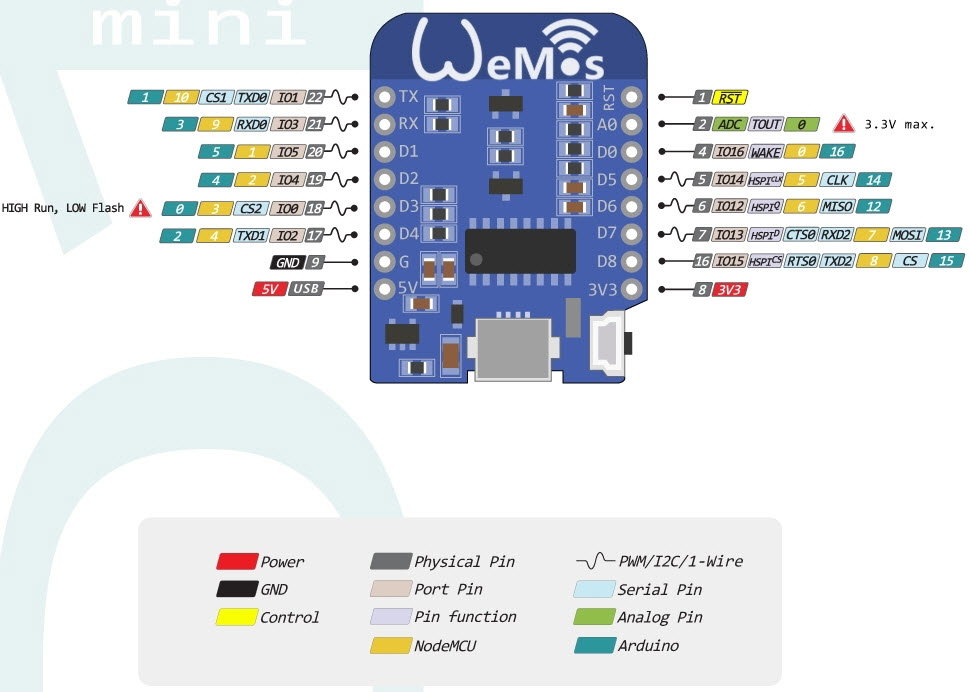
\includegraphics[scale=.6]{d1-mini-esp8266-pinout.jpg}}
                        \end{center}
                        \caption{Chức năng của các chân trên module ESP8266 Wemos D1 (Mini)} \label{Fig:chuc-nang-pin-esp8266-wemos-d1}
                    \end{figure}
            \end{itemize}
    \end{itemize}

\section{Công cụ và ngôn ngữ lập trình cho Module ESP8266}
    \begin{itemize}
        \item Công cụ lập trình: sử dụng Arduino IDE với cấu hình cần thiết.
        \item Ngôn ngữ lập trình: sử dụng ngôn ngữ lập trình Arduino.
    \end{itemize}
\subsection{Cài đặt môi trường lập trình Arduino IDE}
    Truy cập vào địa chỉ https://www.arduino.cc/en/Main/Software để tải phần mềm về sử dụng trên máy tính. Sau khi lựa chọn phiên bản cài đặt phù hợp, chọn JUST DOWNLOAD để tiến hành tải về máy.
\subsection{Cài đặt môi trường lập trình cho ESP8266 trên Arduino IDE}
    Để sử dụng môi trường lập trình Arduino IDE lập trình cho module ESP8266, cần thiết lập theo các bước sau:
        \begin{itemize}
            \item Mở Arduino IDE, chọn File/Preferences được giao diện như \fig{\ref{Fig:Preferences-2-Arduino-IDE}}.
                \begin{figure}[htp]
                    \begin{center}
                        \subfloat[Tab Preferences \label{Fig:Preferences-2-Arduino-IDE}]
                            {
                                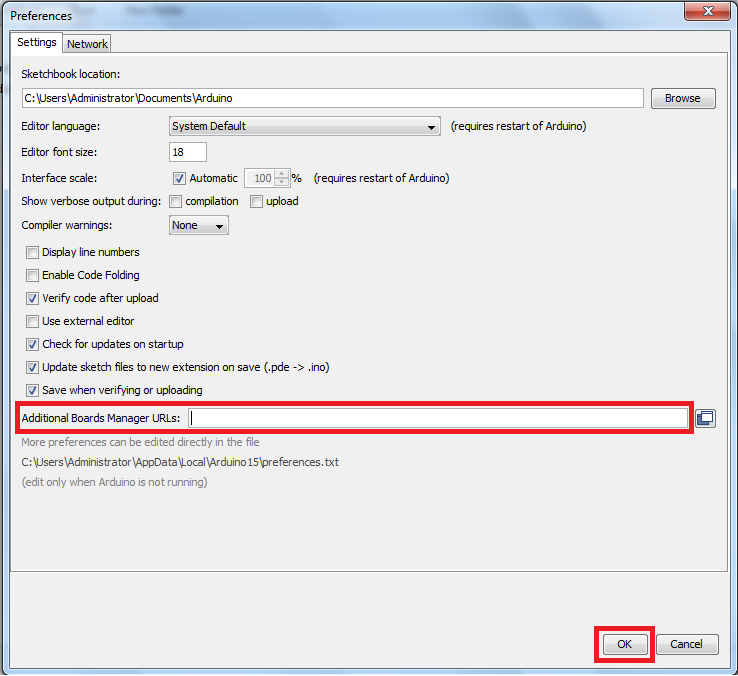
\includegraphics[scale=.35]{arduino-ide-preferences-2.png}
                            }\hspace{.5cm}
                        \subfloat[Điền URLs vào Additional Boards Manager URLs \label{Fig:Preferences-3-Arduino-IDE}]
                            {
                                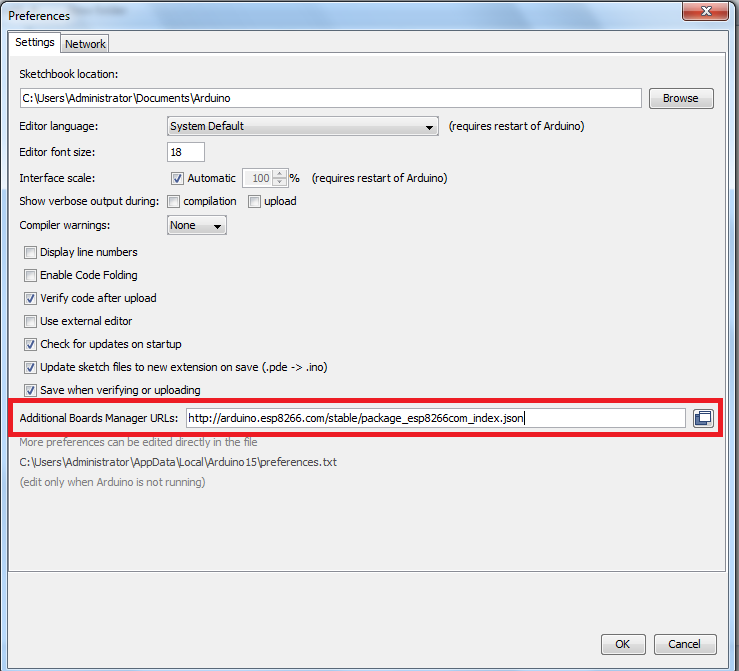
\includegraphics[scale=.35]{arduino-ide-preferences-3.png}
                            }
                    \end{center}
                    \caption{Arduino IDE Preferences}\label{Fig:Preferences-Arduino-IDE}
                \end{figure}
            \item Điền địa chỉ sau vào khung Additional Boards Manager URLs (\fig{\ref{Fig:Preferences-3-Arduino-IDE}}) và chọn OK: http://arduino.esp8266.com/stable/package\_esp8266com\_index.json
            \item Chọn Tool/Board/Boards Manager... Nhập từ khóa esp8266 vào khung tìm kiếm, chọn ESP8266 by ESP8266 Community và nhấn Install để cài đặt. Cài đặt hoàn thành chọn Close (\fig{\ref{Fig:Boards-Manager-Arduino-IDE}}).
                \begin{figure}[htp]
                    \begin{center}
                        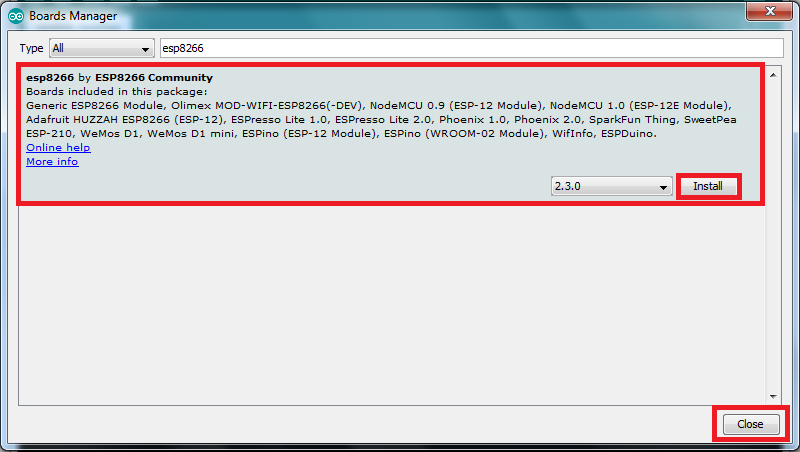
\includegraphics[scale=.58]{arduino-ide-boards-manager-2.png}
                    \end{center}
                    \caption{Arduino IDE Boards Manager -- ESP8266} \label{Fig:Boards-Manager-Arduino-IDE}
                \end{figure}
            \item Chọn Board để nạp chương trình cho ESP8266. Vào Tools, thiết lập các tùy chọn như sau:
                \begin{itemize}
                    \item Board: "WeMos D1 (Retried)".
                    \item CPU Frequency: "80 MHz".
                    \item Flash Size: "4M (3M SPIFFS)".
                    \item Upload Speed: "115200".
                    \item Port: "COM5" (thay đổi tên cổng COM cho phù hợp với từng máy tính).
                    \item Programer AVRISP mkII.
                \end{itemize}
        \end{itemize}

\section{Giao thức SmartConfig kết nối WiFi cho Module ESP8266}
\subsection{Giới thiệu giao thức SmartConfig}
    SmartConfig là một khái niệm được nhắc đến khi muốn cấu hình thông tin cho thiết bị WiFi kết nối nhanh chóng đến Internet nhất từ người dùng bằng chính thiết bị (điện thoại) của họ.

    SmartConfig có thể hiểu là chúng ta gửi thông tin mạng WiFi (bao gồm tên WiFi và password WiFi) cho ESP thông qua smartphone thay cho cách thông thường là phải khai báo thông tin này trong chương trình và nạp firmware xuống.

    SmartConfig có một số lợi ích sau:
        \begin{itemize}
            \item Dễ dàng cấu hình WiFi cho ESP8266 thông qua smartphone.
            \item Không cần phải nạp lại code để cấu hình.
            \item Có thể dùng SmartConfig để cấu hình nhiều thiết bị cùng một lúc.
        \end{itemize}
\subsection{Một số ứng dụng trên điện thoại để thực hiện SmartConfig}
    \begin{itemize}
        \item Sử dụng App ESP Touch (trên iOS) hoặc App ESP SmartConfig (trên Android) để thực hiện kết nối WiFi qua giao thức SmartConfig cho ESP8266.

        \item Ví dụ về cách hoạt động của giao thức ESP Touch gửi thông tin của mạng WiFi cho ESP8266: ESP Touch là protocol được dùng trong SmartConfig để người dùng có thể kết nối tới các phiên bản module ESP8266 thông qua cấu hình đơn giản trên Smartphone. Ban đầu không thể kết nối với ESP8266, nhưng thông qua giao thức ESP TOUCH thì Smartphone sẽ gửi gói UDP tới Access Point (AP) ở đây là ESP8266, mã hóa SSID và mật khẩu thành trường Length trong gói UDP, để ESP8266 có thể hiểu và giải mã được thông tin.
    \end{itemize}
\subsection{Sử dụng App ESP Touch trên iOS thực hiện SmartConfig cho ESP8266}
    \begin{itemize}
        \item Cài đặt App Esptouch cho điện thoại (trên hệ điều hành iOS).
        \item Cách thực hiện kết nối WiFi cho ESP8266 thông qua SmartConfig với App Esptouch:
            \begin{itemize}
                \item Mở App Esptouch (\fig{\ref{Fig:esptouch-1}}), nhập mật khẩu WiFi mà điện thoại đang kết nối vào (\fig{\ref{Fig:esptouch-2}}).
                \item Nhấn Confirm để gửi thông tin của mạng WiFi cho ESP8266 và đợi phản hồi về: nếu kết quả giống \fig{\ref{Fig:esptouch-3}} là ESP8266 kết nối WiFi thành công.
            \end{itemize}
            \begin{figure}[htp]
                \begin{center}
                    \subfloat[Mở App Esptouch \label{Fig:esptouch-1}]
                        {
                            \fbox{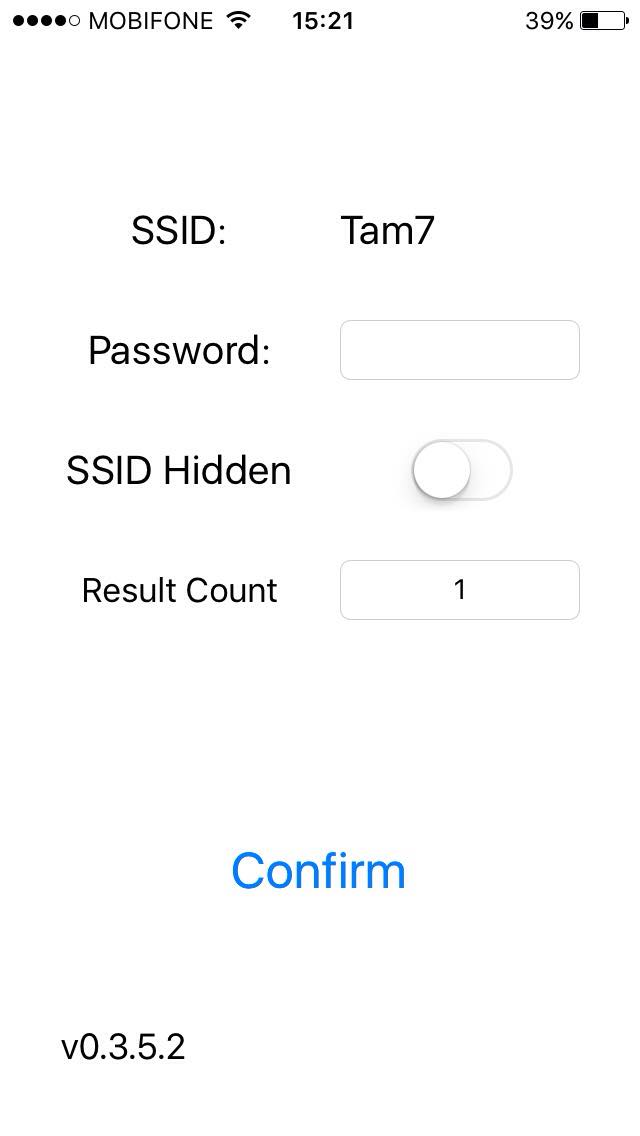
\includegraphics[scale=.2]{esptouch-1}}
                        }
                    \subfloat[Nhập password của mạng WiFi \label{Fig:esptouch-2}]
                        {
                            \fbox{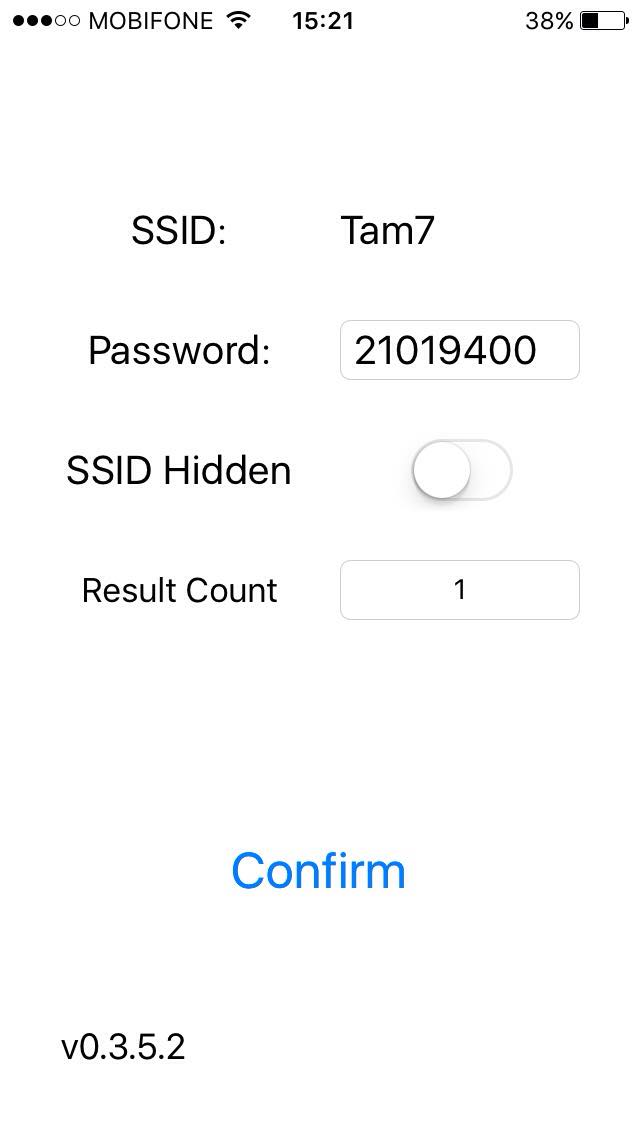
\includegraphics[scale=.2]{esptouch-2}}
                        }
                    \subfloat[Kết nối thành công \label{Fig:esptouch-3}]
                        {
                            \fbox{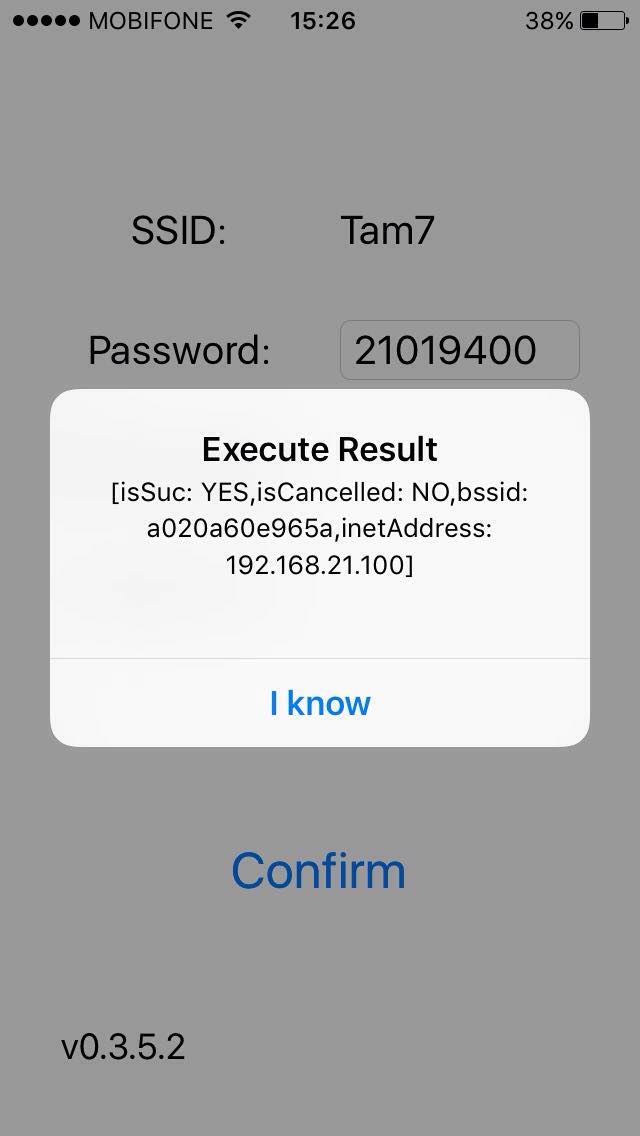
\includegraphics[scale=.2]{esptouch-3}}
                        }
                \end{center}
                \caption{Thực hiện SmartConfig với App Esptouch trên iOS}\label{Fig:smartconfig-esptouch}
            \end{figure}
    \end{itemize}

\newpage
\section{Ứng dụng Blynk trên điện thoại}
\subsection{Giới thiệu}
	Blynk là ứng dụng điện thoại trên hệ điều hành iOS và Android hỗ trợ viết các ứng dụng di động cho các thiết bị thông minh. Ứng dụng cho phép chúng ta dễ dàng kết nối với các mạch tích hợp thông dụng như Arduino, Raspberry Pi, ESP8266, Particle (Photon/SparkCore) và điều khiển thông qua Internet.
\subsection{Cài đặt App Blynk và thư viện Bkynk cho lập trình}
    \begin{itemize}
        \item Tải App Blynk về cài đặt trên điện thoại.
        \item Mở App Blynk và tạo tài khoản sử dụng App.
        \item Tải thư viện Blynk hỗ trợ viết chương trình: github.com/blynkkk/blynk-library
    \end{itemize}
\subsection{Tạo project trong App Blynk}
    Các thuộc tính cần lưu ý: Choose Device (vi điều khiển đang sử dụng), Connection Type (hình thức kết nối để điều khiển, ví dụ là WiFi) và Auth Token (mã xác thực kết nối giữa vi điều khiển và App Blynk).
        \begin{figure}[!ht]
            \begin{center}
                \subfloat[Chọn New Project \label{Fig:blynk-create-project-1}]
                    {
                        \fbox{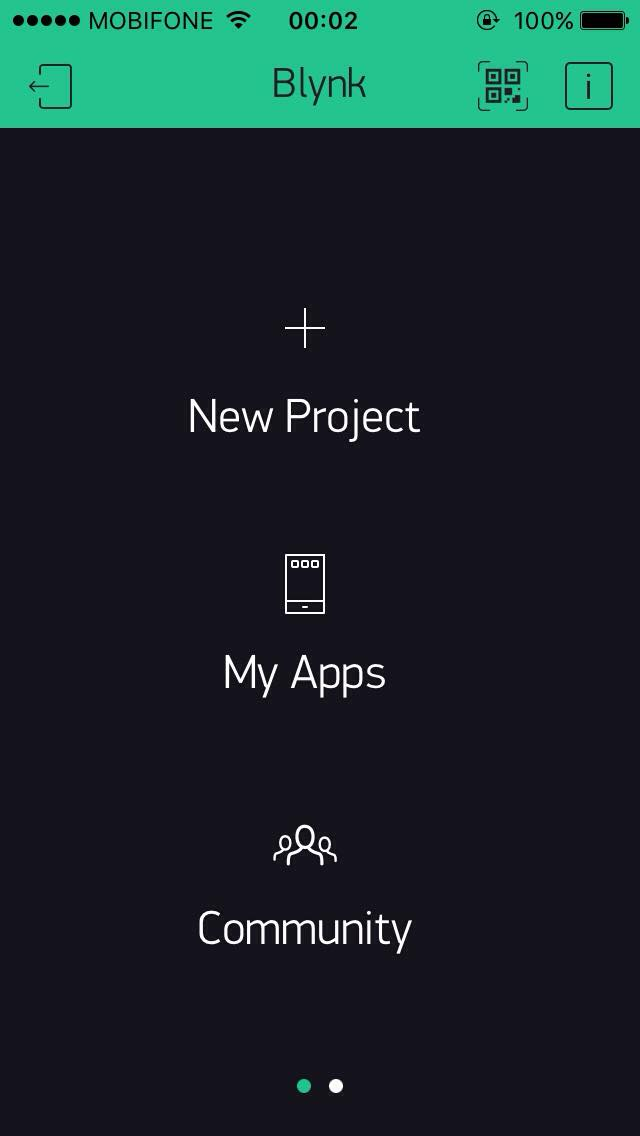
\includegraphics[scale=.2]{create-project-1}}
                    }
                \subfloat[Thay đổi thông tin project \label{Fig:blynk-create-project-2}]
                    {
                        \fbox{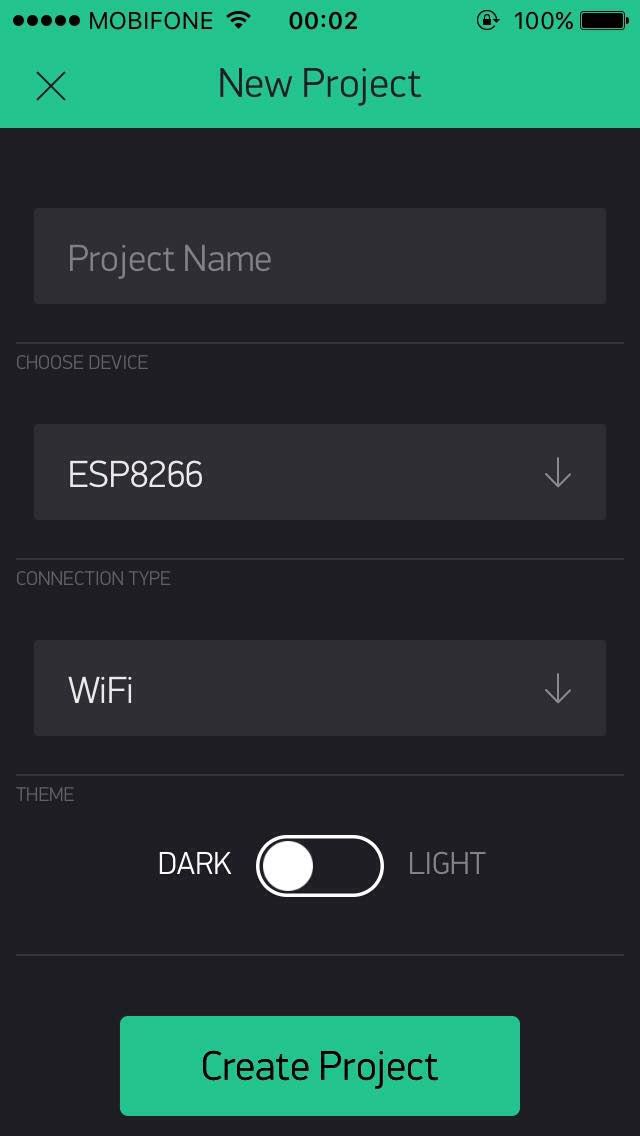
\includegraphics[scale=.2]{create-project-2}}
                    }
                \subfloat[Thông tin project \label{Fig:blynk-create-project-3}]
                    {
                        \fbox{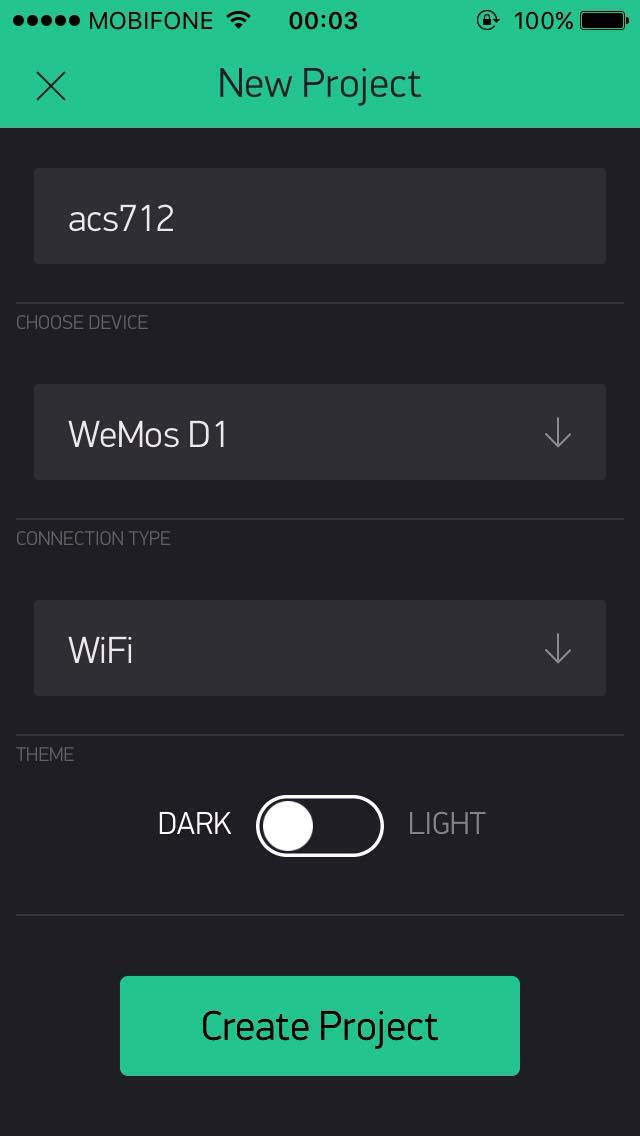
\includegraphics[scale=.2]{create-project-3}}
                    }\\
                \subfloat[Giao diện thiết kế \label{Fig:blynk-create-project-4}]
                    {
                        \fbox{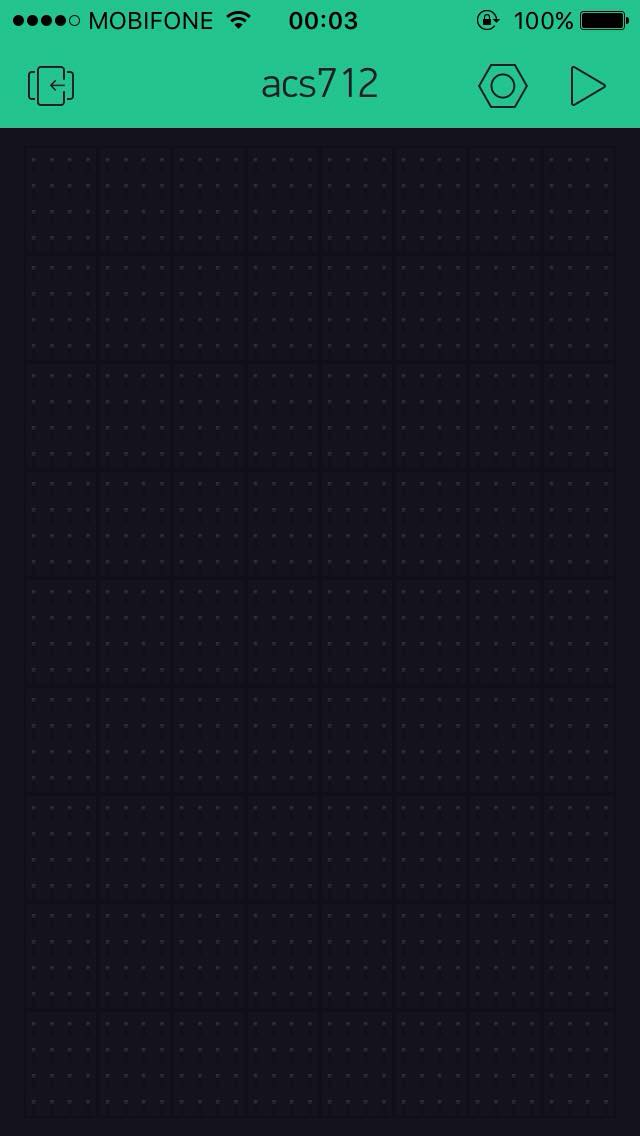
\includegraphics[scale=.2]{create-project-4}}
                    }
                \subfloat[Auth Token của project\label{Fig:blynk-create-project-5}]
                    {
                        \fbox{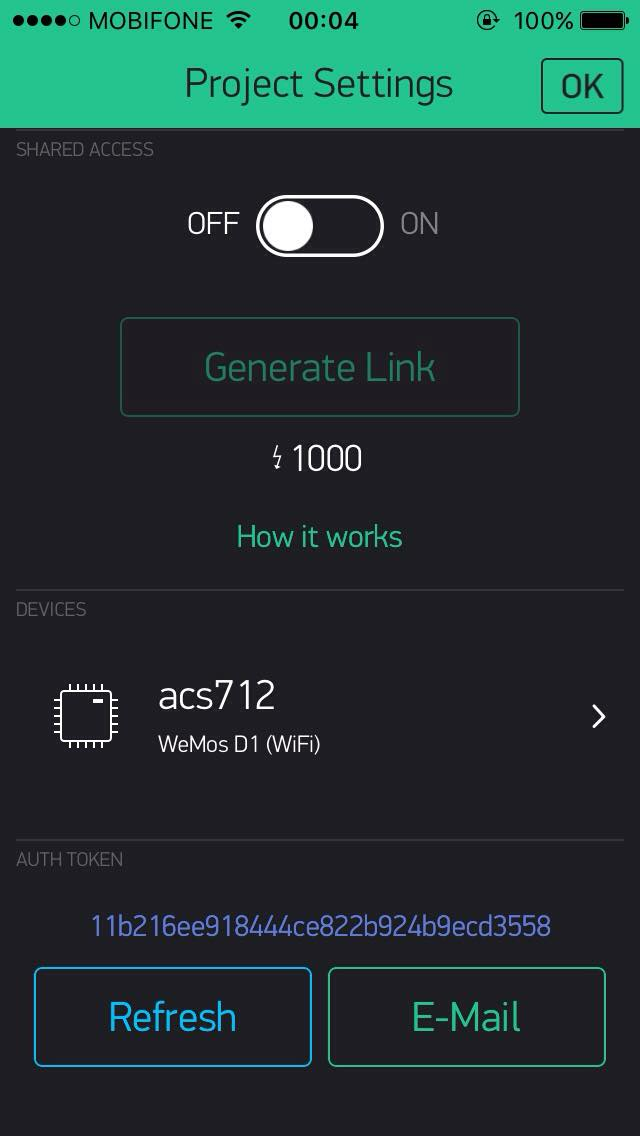
\includegraphics[scale=.2]{create-project-5}}
                    }
            \end{center}
            \caption{Tạo project trong App Blynk}\label{Fig:app-blynk-project}
            % \vspace{-2cm}
        \end{figure}
\subsection{Kết nối giữa các phần tử trên App Blynk và vi điều khiển}
    \begin{itemize}
        \item Để kết nối giữa App Blynk và vi điều khiển: cần chọn đúng Device, Connection Type và lấy Auth Token (được gửi qua Email đăng ký tài khoản).
        \item Để kết nối các phần tử điều khiển trên App Blynk với vi điều khiển: cần biết chính xác PIN (Analog, Digital, Virtual) của các phần tử trên App Blynk để viết chương trình điều khiển tương ứng.
            \begin{itemize}
                \item Các PIN Analog và Digital thường dùng để điều khiển trực tiếp các phần cứng kết nối với vi điều khiển.
                \item Các PIN Vitual để tạo phần cứng ảo hỗ trợ cho vi điều khiển: điều khiển, hiển thị, truyền nhận dữ liệu giữa App và vi điều khiển.
            \end{itemize}
    \end{itemize}

\section{Ứng dụng Web Server Thingspeak}
\subsection{Giới thiệu}
    ThingSpeak là mã nguồn mở cho các ứng dụng Internet of Things -- IoT, hỗ trợ các API lữu trữ, lấy dữ liệu từ thiết bị sử dụng HTTP thông qua kết nối Internet.
\subsection{Cài đặt thư viện Thingspeak cho lập trình}
    Tải thư viện Thingspeak hỗ trợ viết chương trình: github.com/mathworks/thingspeak-arduino
\subsection{Tạo tài khoản sử dụng và tạo project trên Thingspeak}
    \begin{figure}[htp]
        \begin{center}
            \fbox{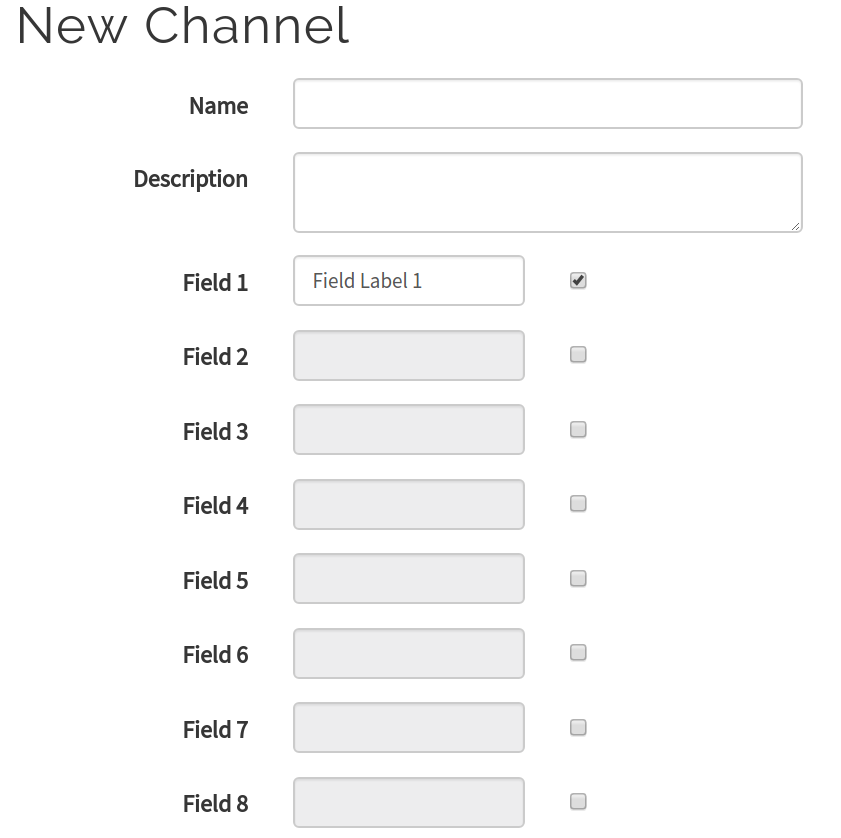
\includegraphics[scale=.3]{create-project}}
        \end{center}
        \caption{Các Field dùng lưu trữ dữ liệu trên Thingspeak} \label{Fig:thingspeak-create-project}
    \end{figure}
    \begin{itemize}
        \item Truy cập vào địa chỉ thingspeak.com, tạo tài khoản sử dụng Thingspeak.
        \item Chọn New Channel để tạo project mới: đặt tên cho project, thông tin mô tả cho project, tên cho các Field và chọn Save Channel. Các Field 1 đến Field 8 là các field dùng để lưu trữ dữ liệu từ vi điều khiển gửi lên Thingspeak (\fig{\ref{Fig:thingspeak-create-project}}).
        \item Để kết nối giữa Web Server Thingspeak và vi điều khiển cần có Channel ID và Write API Key (vào tab API Keys để lấy Write API Key).
    \end{itemize}
\subsection{Cách giao tiếp vi điều khiển và Web Server Thingspeak}
    Sử dụng phương thức POST/GET/\ldots trong giao thức HTTP để gửi dữ liệu lên Web Server Thingspeak.

\section{Cảm biến dòng điện ACS712}
\subsection{Giới thiệu}
    Cảm biến dòng điện ACS712 là IC cảm biến dòng tuyến tính dựa trên hiệu ứng Hall. Cảm biến xuất ra tín hiệu analog Vout biến đổi tuyến tính theo sự thay đổi của dòng điện được lấy mẫu thứ cấp DC (hoặc AC), trong phạm vi đã cho. Tụ (Cf theo sơ đồ) được dùng với mục đích chống nhiễu và có giá trị tùy thuộc vào từng mục đích sử dụng.
        \begin{figure}[htp]
            \begin{center}
                \subfloat[]
                    {
                        \fbox{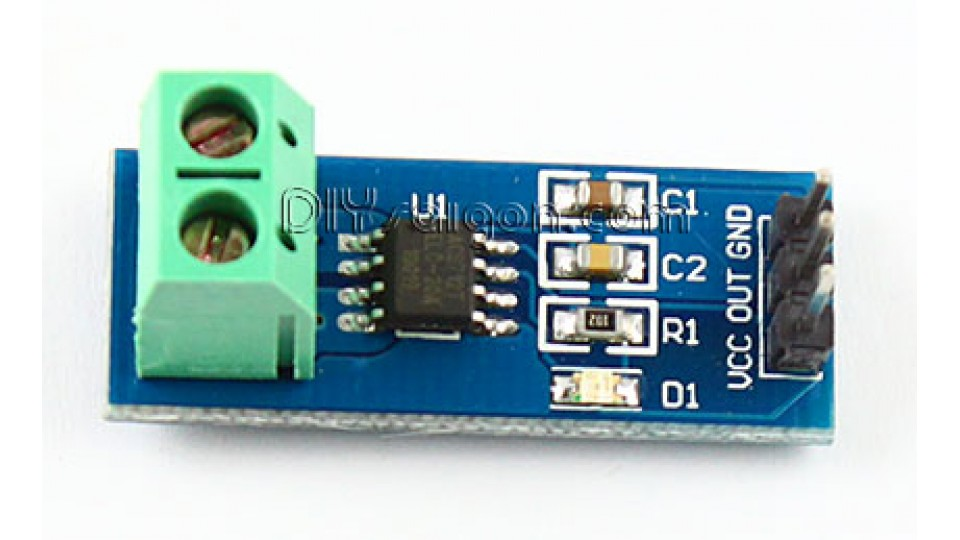
\includegraphics[scale=.28]{acs712}}
                    }
                \subfloat[]
                    {
                        \fbox{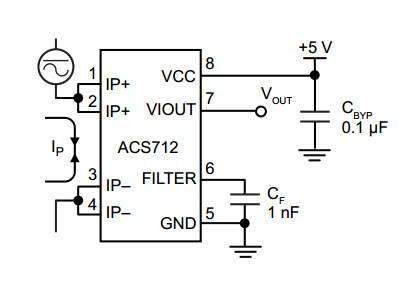
\includegraphics[scale=.5]{acs712-schem}}
                    }
            \end{center}
            \caption{Cảm biến dòng ACS712} \label{Fig:acs712}
        \end{figure}
\subsection{Đặc điểm của cảm biến}
    \begin{itemize}
        \item Thời gian tăng của đầu ra để đáp ứng với đầu vào là 5$\mu$s.
        \item Điện trở dây dẫn trong là 1.2m$\Omega$.
        \item Điện áp hoạt động 5V.
        \item Độ nhạy đầu ra từ 63 -- 190mV/A ứng với từng loại cảm biến: 64 -- 68 mV/A (loại 30A); 96 -- 104mV/A (loại 20A) và 180 -- 190mV/A (loại 5A).
        \item Điện áp ra ổn định.
    \end{itemize}
\subsection{Cách sử dụng module cảm biến dòng ACS712}
    \begin{itemize}
        \item Đo dòng điện DC:
            \begin{itemize}
                \item Khi đo DC phải mắc tải nối tiếp $Ip+$ và $Ip-$ đúng chiều, dòng điện đi từ $Ip+$ đến $Ip-$ để Vout ra mức điện thế 2.5V đến 5V tương ứng dòng 0 đến $I_{\textrm{đmcb}}$ (dòng điện định mức mà cảm biến đo được), nếu mắc ngược Vout sẽ ra điện thế 2.5V đến 0V tương ứng với 0A đến $-I_{\textrm{đmcb}}$.
                \item Cấp nguồn 5V cho module khi chưa có dòng $Ip$ (chưa có tải mắc nối tiếp với domino), thì Vout là 2.5V. Khi dòng $Ip$ (dòng của tải) bằng $I_{\textrm{đmcb}}$ thì Vout là 5V, Vout sẽ tuyến tính với dòng $Ip$, trong khoảng 2.5V đến 5V tương ứng với dòng 0 đến $I_{\textrm{đmcb}}$.
                \item Công thức tính dòng điện DC (với $V_m$ là độ nhạy ứng với từng loại cảm biến dòng ACS712 được trình bày ở trên):
                    \begin{align*}
                        V_{(mV)} = \dfrac{adc \times 5000.0}{1024.0};\quad I_{(mA)} = \dfrac{V - 2500}{V_m} \quad \textrm{(với } V_m \textrm{ là độ nhạy)}
                    \end{align*}
            \end{itemize}

        \item Đo dòng điện AC:
            \begin{itemize}
                \item Khi đo dòng điện AC, do dòng điện AC không có chiều nên không cần quan tâm chiều.
                \item Cấp nguồn 5V cho module khi chưa có dòng $Ip$ (chưa có tải mắc nối tiếp với domino), thì Vout là 2.5V. khi có dòng xoay chiều $Ip$ (dòng AC) do dòng xoay chiều độ lớn thay đổi liên tục theo hàm sin, nên điện thế Vout sẽ là điện thế xoay chiều hình sin có độ lớn tuyến tính với dòng điện AC, 0 đến 5V (thế xoay chiều) tương ứng với $-I_{\textrm{đmcb}}$ đến $+I_{\textrm{đmcb}}$ (dòng xoay chiều).
                \item Công thức tính dòng điện AC (với $V_m$ là độ nhạy ứng với từng loại cảm biến dòng ACS712 được trình bày ở trên):
                    \begin{align*}
                        V_{(mV)} = \dfrac{adc_{MaxPoint} \times 5000.0}{1024.0};\quad I_{(mA)} = \dfrac{V - 2500}{\sqrt{2}V_m} \quad \textrm{(với } V_m \textrm{ là độ nhạy)}
                    \end{align*}
            \end{itemize}
    \end{itemize}

\section{Xác định công suất, điện năng tiêu thụ của phụ tải xoay chiều một pha dựa vào dòng điện qua tải và thời gian hoạt động của tải}
    \begin{itemize}
        \item Công suất tiêu thụ của phụ tải xoay chiều một pha: $P = UI\cos \varphi$.
        \item Giá trị dòng điện đo được là giá trị tức thời: $I_{i}$.
        \item Công suất tức thời: $P = U_iI_i\cos \varphi_i$
        \item Công suất trung bình có thể xác định gần đúng bằng công thức sau:
            \begin{align*}
                P_{tb} = \dfrac{1}{n}\sum^n_{i=1}P_i
            \end{align*}
        \item Do cảm biến ACS712 chỉ có thể được dòng điện đi qua phụ tải, không đo được điện áp cấp cho phụ tải. Để đơn giản chọn điện áp $U$ cấp cho phụ tải một pha và hệ số công suất $\cos \varphi$ là không đổi, khi đó ta có:
            \begin{align*}
                P_{tb} = \dfrac{1}{n}\sum^n_{i=1}P_i = \dfrac{U\cos \varphi}{n}\sum^n_{i=1}I_i
            \end{align*}
            Khi tính toán, có thể chọn gần đúng $U = 220V$ và $\cos \varphi = 0.86$
        \item Điện năng tiêu thụ của phụ tải: $A = \sum^m_{j=1} P_{tb_j}t_j$ với $P_{tb_j}$ là công suất trung bình trong thời gian phụ tải hoạt động $t_j$.
    \end{itemize}
